\section{Assessing the Performance Impact}

\label{sec:predictimprove}

Fixing false sharing problems can be non-trivial, even with precise information about a particular false sharing problem. Even worse, fixing false sharing problems does not necessarily bring the performance improvement. For example, existing tools report a big number of cache invalidations related to false sharing in word\_count or reverse\_index applications, but fixing them brings negligible performance improvement~\cite{Sheriff, Predator}. Zhao et. al. even observed that fixing may even slowdown a program because of excessive memory consumption or the lose of locality~\cite{qinzhao}. Reporting insignificant false sharing instances are not false positives, but that increases manual burden for programmers.

To resolve this problem, \cheetah{} makes the first attempt to quantitatively assess the potential performance gain of fixing a particular false sharing problem. So that programmers can focus on severe problems only, avoiding unnecessary manual effort.

\cheetah{}'s assessment is based on the following observations:

\begin{itemize}
\item {\bf Observation 1:} the sampling is evenly distributed over the whole execution. Thus, we can  use the results of sampling to represent the whole execution. The similar ideas has been widely used by the exiting work like Oprofile and Gprof to identify the hotspots of function calls and code~\cite{oprofile, DBLP:conf/sigplan/GrahamKM82}.

\item {\bf Observation 2:} PMU hardware provides the latency information (e.g. cycles) of each memory load operation. We also observed that the latency of accessing falsely shared objects is significantly higher than that of normal accesses. 

\end{itemize}

Based on these two observations, {\bf we propose to use the sampled cycles of an execution to represent the execution time or the runtime}. 

\cheetah{} predicts the performance impact of an falsely-shared object $O$ in three steps listed as follows. 

\begin{itemize}
\item \cheetah{} first evaluates how much performance impact on accesses on this object $O$, as discussed in Section~\ref{sec:impactobject}. 

\item Then \cheetah{} assesses how much performance impact on the related threads by fixing this false sharing problem, which is discussed in Section~\ref{sec:impactthread}. 
 
\item In the end, \cheetah{} assesses how much performance impact on the application, seen in Section~\ref{sec:impactapp}. 
\end{itemize}


\subsection{Impact on Accesses of the Object}
\label{sec:impactobject}

To assess the performance impact of fixing a falsely-shared object $O$, \cheetah{} has to collect the following information. 
 
\begin{itemize}
\item $Cycles_O$: total cycles on a falsely-shared object $O$.
\item $Accesses_O$: total number of accesses on the object $O$.  
\item $AverageCycles_{nofs}$: the average cycles of every memory access on non-falsely-shared (abbreviated as ``non-FS'') objects. \cheetah{} utilizes the average cycles of each access that happened in the serial phases as the $AverageCycles_{nofs}$. There is no false sharing problem in serial phases since there is only one thread in total.  

\end{itemize}

Based on the information, \cheetah{} predicts the total cycles of all accesses after the fix, noted as $PredictCycles_{O}$, to be equal to  
 the product of $Accesses_O$ and $AverageCycles_{nofs}$, as shown in EQ.(\ref{eq:predictedcyclesofo}).
 
\begin{equation}
\label{eq:predictedcyclesofo}
 PredictCycles_{O} = (AverageCycles_{nofs} * Accesses_O);
\end{equation} 
 
Here, we assume that the number of accesses after fixing keeps the same (e.g. $Accesses_O$), and the best latency of each access after fixing the false sharing problem of the object $O$ will be equal to $AverageCycles_{nofs}$. But in reality, the cycle of every access can be larger than $AverageCycles_{nofs}$ since fixing false sharing problems may cause excessive memory consumption or the lose of locality~\cite{qinzhao}. Thus, our prediction will provide an upper bound of performance improvement. 


\subsection{Impact on Related Threads}
\label{sec:impactthread}

After getting the $PredictCycles_{O}$, we will assess the possible execution time of different threads by fixing the false sharing problem of Object $O$. 

To achieve this target, \Cheetah{} will collect the following information of every thread: the execution time -- $RT_{thread}$, the total number of accesses $Accesses_{thread}$, and the total cycles of all memory accesses in this thread -- $Cycles_{thread}$.

In real implementation, \cheetah{} intercepts the creation of different threads by passing a custom function as the start routine. In this custom function, \cheetah{} gets the timestamp before and after running the actual thread function so that it can compute the execution time of a thread ($RT_{thread}$). To gather the number of accesses and cycles of every thread, \cheetah{} makes every thread to respond the signal handler and records the number of accesses and cycles correspondingly when every memory access is sampled, as described in Section~\ref{sec:perfcounter}. 

After that, \cheetah{} first predicts the new cycles of related thread ($PredictCycles_{thread}$) as the EQ.(\ref{eq:predictedcyclesofthread}).

\begin{equation}
\label{eq:predictedcyclesofthread}
 PredictCycles_{thread} = Cycles_{thread} - Cycles_{O} + PredictCycles_{O} 
\end{equation} 
 

Then based on this, \cheetah{} assesses the predicted runtime of a thread--- $PredictRT_{thread}$--- as the EQ.(\ref{eq:predictedrtofthread}). In this step, we assume that {\bf the execution time is proportional to the cycles of accesses}: the less of cycles means the less of the execution time.  

\begin{equation}
\label{eq:predictedrtofthread}
 PredictRT_{thread} = (PredictCycles_{thread}/Cycles_{thread}) * RT_{thread} 
\end{equation} 

\subsection{Impact on the Application}
\label{sec:impactapp}

After getting the predicted execution time--$PredictRT_{thread}$-- after fixing a false sharing problem, we will assess how it will finally change the performance of the application. 

This a very challenging topic.  We have to monitor the execution of different threads. For example, if a thread is not in the critical path of the performance, then fixing false sharing problems in this thread will not have an observed impact on the final performance. The assessment can become even more complicated if there are some nested threads in the application. 

To simplify our prediction and verify the idea, \cheetah{} focuses on its assessment on the normal fork-join model, which is the most important and widely used model. A basic example of fork-join model is shown in  Figure~\ref{fig:forkjoinmodel}. All applications that we evaluated in this paper, including all benchmarks in phoenix and parsec benchmarks suite, utilizes this fork-join model. 

\begin{figure*}[ht!]
\begin{center}
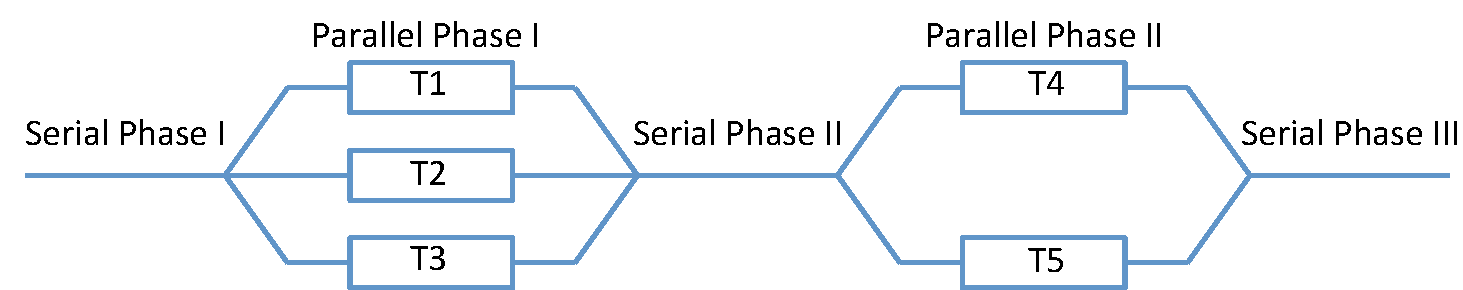
\includegraphics[width=6in]{figure/forkjoin}
\end{center}
\caption{The fork-join model that \Cheetah{} currently focuses on to assess the impact of false sharing instances. 
\label{fig:forkjoinmodel}}
\end{figure*}

In order to identify whether an execution belongs to the fork-join model as Figure~\ref{fig:forkjoinmodel}, \cheetah{} has to keep track of creation creations and thread joins. For example, the main thread will enter the parallel phase I after \cheetah{} intercepts the first thread creation. The execution will leave the parallel phase I after all children threads that are created has been joined successfully. 

\Cheetah{} collects the execution time of different serial and parallel phases using RDTSC (ReaD-Time Stamp Counter) on X86 machines. The difference between the stopping point and the starting point will be considered as the length of a phase. 

After having the information of execution time of different phases, \cheetah{} can predict the final performance impact on the application. The basic idea is to predict the execution time of different threads as described in Section~\ref{sec:impactthread}, then recompute the length of each phase and the total time. After that, we will compute the final performance improvement using the following equation. 

\cheetah{} will compute the potential performance improvement based on EQ.(\ref{eq:improvement}), where runtime is denoted by $RT$.

\begin{equation}
\label{eq:improvement}
Perf_{improve}=RT_{actual}/RT_{predict}
\end{equation}

We will uses an example to show that. For example, there is a false sharing problem that will involved in the $T1$ and $T2$ of Figure~\ref{fig:forkjoinmodel}, but not other threads.  We will assess the possible runtime of $PredictRT_{T1}$ and $PredictRT_{T2}$. Then we checked that whether these predicted runtime will affect the runtime of parallel phase I by checking whether these two runtime are less than the runtime of $T3$ at first. If it won't, then fixing the false sharing problem won't affect the final performance. 
Otherwise, we have to recompute the length of parallel phase I, while the length of other phases will keep the same. By doing that, we will get a new runtime for the application. Using the EQ.(\ref{eq:improvement}), we can compute the potential performance improvement of this application by fixing the false sharing problems related to the thread $T1$ and $T2$. 

Although  \cheetah{} only focuses on the fork-join model, the idea of predicting false sharing impact can be applied to other execution models, but with more complexity. We further verified the precision of our assessment in Section~\ 








